%---------------------------------------------------------%
%______//------             GAC             ------\\______%
%______||------         Chapitre 7          ------||______%
%______\\------      Graphes de Cayley      ------//______%
%---------------------------------------------------------%

\chapter{Graphes de Cayley (groupes comme espaces métriques)}
\label{sec:graphes-de-Cayley}

  Soit $G$ un groupe, $S \subset G$ une partie symétrique ($s \in S \Rightarrow s^{-1} \in S$) et $1 \notin
  S$.

  \begin{defi} \index{Graphe!de Cayley}
    Le \emph{graphe de Cayley}, noté $\Gamma(G, S)$ est le graphe dont l'ensemble des sommets est $G$ et
    l'ensemble des arêtes est $E = \{(x,y) | xy^{-1} \in S \iff \exists s \in S\ :\ y = xs\}$.

    Deux sommets sont \emph{voisins}, et on les notes $x \sim y$, si $y$ s'obtient à partir de $x$ par
    multiplication par un élément de $S$.
  \end{defi}

  \begin{exs}
    \begin{enumerate}
    \item Soit $G = \Z/6\Z$ et $S = \{x, x^{-1}\}$, pour $x = 1$ et $x^{-1} = 5$.
      \begin{center}
        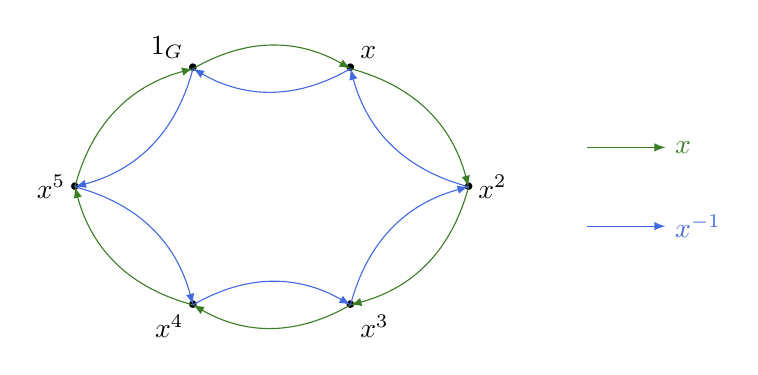
\begin{tikzpicture}
          % Nodes
          \draw (0,0) node[scale=0.7]{$\bullet$} node[above left]{$1_G$};
          \draw (2,0) node[scale=0.7]{$\bullet$} node[above right]{$x$};
          \draw (3.5,-1.5) node[scale=0.7]{$\bullet$} node[right]{$x^2$};
          \draw (2,-3) node[scale=0.7]{$\bullet$} node[below right]{$x^3$};
          \draw (0,-3) node[scale=0.7]{$\bullet$} node[below left]{$x^4$};
          \draw (-1.5,-1.5) node[scale=0.7]{$\bullet$} node[left]{$x^5$};
          % Edges (x)
          \draw[->, >=latex, color=OliveGreen] (0,0) to[bend left] (2,0);
          \draw[->, >=latex, color=OliveGreen] (2,0) to[bend left] (3.5, -1.5);
          \draw[->, >=latex, color=OliveGreen] (3.5,-1.5) to[bend left] (2, -3);
          \draw[->, >=latex, color=OliveGreen] (2,-3) to[bend left] (0,-3);
          \draw[->, >=latex, color=OliveGreen] (0,-3) to[bend left] (-1.5, -1.5);
          \draw[->, >=latex, color=OliveGreen] (-1.5,-1.5) to[bend left] (0,0);
          % Edges (x^-1)
          \draw[<-, >=latex, color=RoyalBlue] (0,0) to[bend right] (2,0);
          \draw[<-, >=latex, color=RoyalBlue] (2,0) to[bend right] (3.5, -1.5);
          \draw[<-, >=latex, color=RoyalBlue] (3.5,-1.5) to[bend right] (2, -3);
          \draw[<-, >=latex, color=RoyalBlue] (2,-3) to[bend right] (0,-3);
          \draw[<-, >=latex, color=RoyalBlue] (0,-3) to[bend right] (-1.5, -1.5);
          \draw[<-, >=latex, color=RoyalBlue] (-1.5,-1.5) to[bend right] (0,0);
          % Legend
          \draw[->, >=latex, color=OliveGreen] (5, -1) to (6,-1) node[right]{$x$};
          \draw[->, >=latex, color=RoyalBlue] (5,-2) to (6,-2) node[right]{$x^{-1}$};
        \end{tikzpicture}
      \end{center}

    \item Soit $G = \Z/6\Z$ et $S = \{2, -2\}$.
      \begin{center}
        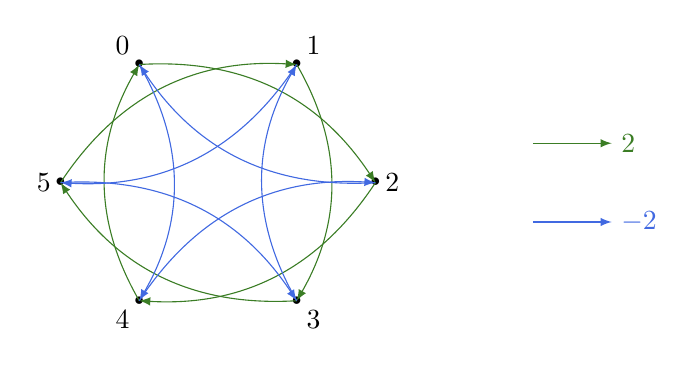
\begin{tikzpicture}
          % Nodes
          \node[scale=0.7] (0) at (0,0){$\bullet$};
          \node[scale=0.7] (1) at (2,0){$\bullet$};
          \node[scale=0.7] (2) at (3,-1.5){$\bullet$};
          \node[scale=0.7] (3) at (2,-3){$\bullet$};
          \node[scale=0.7] (4) at (0,-3){$\bullet$};
          \node[scale=0.7] (5) at (-1,-1.5){$\bullet$};
          % Nodes labels
          \draw (0) node[above left]{$0$};
          \draw (1) node[above right]{$1$};
          \draw (2) node[right]{$2$};
          \draw (3) node[below right]{$3$};
          \draw (4) node[below left]{$4$};
          \draw (5) node[left]{$5$};
          % Edges (2)
          \draw[->, >=latex, color=OliveGreen] (0.center) to[bend left] (2.center);
          \draw[->, >=latex, color=OliveGreen] (2.center) to[bend left] (4.center);
          \draw[->, >=latex, color=OliveGreen] (4.center) to[bend left] (0.center);
          \draw[->, >=latex, color=OliveGreen] (1.center) to[bend left] (3.center);
          \draw[->, >=latex, color=OliveGreen] (3.center) to[bend left] (5.center);
          \draw[->, >=latex, color=OliveGreen] (5.center) to[bend left] (1.center);
          % Edges (-2)
          \draw[<-, >=latex, color=RoyalBlue] (0.center) to[bend right] (2.center);
          \draw[<-, >=latex, color=RoyalBlue] (2.center) to[bend right] (4.center);
          \draw[<-, >=latex, color=RoyalBlue] (4.center) to[bend right] (0.center);
          \draw[<-, >=latex, color=RoyalBlue] (1.center) to[bend right] (3.center);
          \draw[<-, >=latex, color=RoyalBlue] (3.center) to[bend right] (5.center);
          \draw[<-, >=latex, color=RoyalBlue] (5.center) to[bend right] (1.center);
          % legend
          \draw[->, >=latex, color=OliveGreen] (5, -1) to (6,-1) node[right]{$2$};
          \draw[->, >=latex, color=RoyalBlue] (5,-2) to (6,-2) node[right]{$-2$};
        \end{tikzpicture}
      \end{center}

    \item Soit $G = \Z/6\Z$ et $S = \{3 = -3\}$.
      \begin{center}
        \begin{tikzpicture}
          % Nodes
          \node[scale=0.7] (0) at (0,0){$\bullet$};
          \node[scale=0.7] (1) at (2,0){$\bullet$};
          \node[scale=0.7] (2) at (3,-1.5){$\bullet$};
          \node[scale=0.7] (3) at (2,-3){$\bullet$};
          \node[scale=0.7] (4) at (0,-3){$\bullet$};
          \node[scale=0.7] (5) at (-1,-1.5){$\bullet$};
          % Nodes labels
          \draw (0) node[above left]{$0$};
          \draw (1) node[above right]{$1$};
          \draw (2) node[right]{$2$};
          \draw (3) node[below right]{$3$};
          \draw (4) node[below left]{$4$};
          \draw (5) node[left]{$5$};
          % Edges (3)
          \draw[<->, >=latex, color=OliveGreen] (0.center) to (3.center);
          \draw[<->, >=latex, color=OliveGreen] (1.center) to (4.center);
          \draw[<->, >=latex, color=OliveGreen] (2.center) to (5.center);
        \end{tikzpicture}
      \end{center}

    \item Soit $G = \Z/6\Z$ et $S = \{2, -2, 3 = -3\}$.
      \begin{center}
        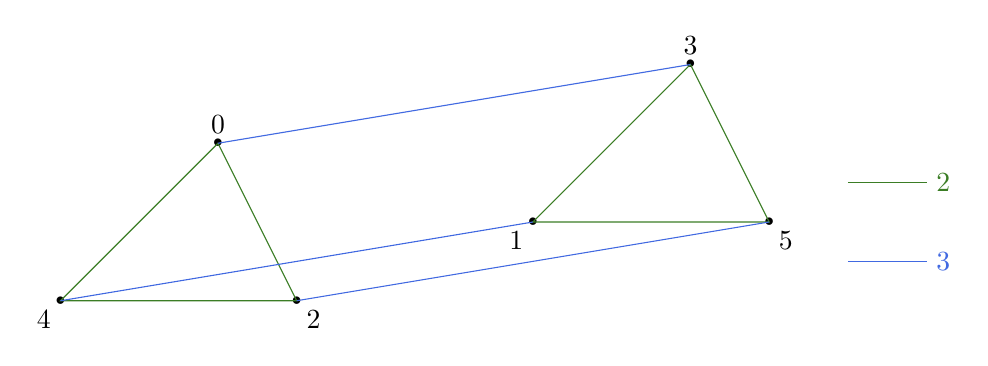
\begin{tikzpicture}
          % Nodes
          \node[scale=0.7] (0) at (0,0){$\bullet$};
          \node[scale=0.7] (2) at (1,-2){$\bullet$};
          \node[scale=0.7] (4) at (-2,-2){$\bullet$};
          \node[scale=0.7] (3) at (6,1){$\bullet$};
          \node[scale=0.7] (5) at (7,-1){$\bullet$};
          \node[scale=0.7] (1) at (4,-1){$\bullet$};
          % Nodes labels
          \draw (0) node[above]{$0$};
          \draw (1) node[below left]{$1$};
          \draw (2) node[below right]{$2$};
          \draw (3) node[above]{$3$};
          \draw (4) node[below left]{$4$};
          \draw (5) node[below right]{$5$};
          % Edges
          \draw[color=OliveGreen] (0.center) to (2.center) to (4.center) to cycle;
          \draw[color=OliveGreen] (3.center) to (5.center) to (1.center) to cycle;
          \draw[color=RoyalBlue] (0.center) to (3.center);
          \draw[color=RoyalBlue] (2.center) to (5.center);
          \draw[color=RoyalBlue] (4.center) to (1.center);
          % Legend
          \draw[color=OliveGreen] (8, -0.5) to (9,-0.5) node[right]{$2$};
          \draw[color=RoyalBlue] (8,-1.5) to (9,-1.5) node[right]{$3$};
        \end{tikzpicture}
      \end{center}

    \item Soit $G = \Z$ et $S = \{1, -1\}$.
      \begin{center}
        \begin{tikzpicture}
          \foreach \n in {-4, -3, ..., 4}{
            \node[scale=0.7] (\n) at (\n, 0){$\bullet$};
            \draw (\n) node[above]{$\n$};
            \draw[->, >=latex, color=OliveGreen] (\n.center) to node[scale=0.7, midway, above]{$1$} ($(\n) + (1,0)$.center);
          }
          \draw (5, 0) node[right]{$\Z$};
        \end{tikzpicture}
      \end{center}

    \item Soit $G = \Z^2$ et $S = \{(\pm 1, 0), (0, \pm 1)\}$.
      \begin{center}
        \begin{tikzpicture}
          \foreach \i in {-2, -1, ..., 2} {
            \foreach \j in {-2, -1, ..., 2} {
              \draw[->, >=latex, color=OliveGreen] (\i, \j) to ($(\i, \j) + (1, 0)$);
              \draw[->, >=latex, color=RoyalBlue] (\i, \j) to ($(\i, \j) + (0, 1)$);
            }
          }
          \draw (0,0) node[scale=0.7, below left]{$(0,0)$};
        \end{tikzpicture}
      \end{center}

    \item Soit $G = \F_2 = \F(a,b)$ le groupe libre avec 2 générateurs et soit $S = \{a^{\pm 1}, b^{\pm 1}\}$.
      \begin{center}
        \begin{tikzpicture}
          \draw l-system [l-system={cayley, axiom=[A] [+A] [-A] [++A], step=3cm, order=4}];
        \end{tikzpicture}
        Source:
        \href{http://tex.stackexchange.com/questions/222881/cayley-graph-of-free-group-in-tikz}{tex.stackexchange}
        (ça vaut la peine de jeter un oeil aux jolis graphs :))
      \end{center}
    \end{enumerate}
  \end{exs}

  \begin{propri}
    \begin{enumerate}
    \item $\Gamma(G,S)$ est $k$-régulier, où $k = |S|$ (c'est-à-dire tout sommet a $k$ voisins).
    \item $\Gamma(G,S)$ et connexe $\iff$ $S$ engendre $G$.
    \end{enumerate}
  \end{propri}

  \begin{defi} \index{Arbre}
    Un \emph{arbre} un graphe connexe sans chemins fermés.
  \end{defi}

  \begin{prop}
    Soit $G$ un groupe et $S \subseteq G$ un ensemble. Alors $G \cong \F(S)$ (le groupe libre sur $S$) si et
    seulement si $\Gamma(G, S)$ est un arbre.
  \end{prop}


  \begin{defi}
    Soient $\Gamma_1 = (V_1, E_1)$ et $\Gamma_2 = (V_2, E_2)$ deux graphes. Un \emph{morphisme de graphe}
    \index{Morphisme!de graphe} est une application $\phi: \Gamma_1 \to \Gamma_2$, $\phi \big|_V : V_1 \to
    V_2$, $\phi \big|_E : E_1 \to E_2$ telle que $(\phi(v), \phi(v')) \in E_2 \iff (v, v') \in E_1$.

    \begin{center}
      \begin{tikzpicture}
        % Nodes
        \node[scale=0.7] (1) at (0,0){$\bullet$};
        \node[scale=0.7] (2) at (-1,-1){$\bullet$};
        \node[scale=0.7] (3) at (-2,-2){$\bullet$};
        \node[scale=0.7] (4) at (1,-1){$\bullet$};
        \node[scale=0.7] (5) at (2,-2){$\bullet$};
        \node[scale=0.7] (a) at (5,0){$\bullet$};
        \node[scale=0.7] (b) at (5,-1){$\bullet$};
        \node[scale=0.7] (c) at (5,-2){$\bullet$};
        % Nodes labels
        \draw (1) node[above]{$1$};
        \draw (2) node[left]{$2$};
        \draw (3) node[left]{$3$};
        \draw (4) node[right]{$4$};
        \draw (5) node[right]{$5$};
        \draw (a) node[right]{$a$};
        \draw (b) node[right]{$b$};
        \draw (c) node[right]{$c$};
        % name of graphs
        \draw (0,  1) node{$\Gamma_1$};
        \draw (5, 1) node{$\Gamma_2$};
        % Edges
        \draw[color=OliveGreen] (1.center) to (2.center) to (3.center);
        \draw[color=OliveGreen] (1.center) to (4.center) to (5.center);
        \draw[color=OliveGreen] (a.center) to (b.center) to (c.center);
        % morphism:
        \draw (8, 0) node{$\phi: 1 \mapsto a$};
        \draw (8, -1) node{$2 \mapsto b,\ 4 \mapsto b$};
        \draw (8, -2) node{$3 \mapsto c,\ 5 \mapsto c$};
        % note
        \draw (0, -3) node{Respecte le voisinage car $\phi((1,2)) = (\phi(1), \phi(2)) = (a,b)$};
      \end{tikzpicture}
    \end{center}

    Si $\phi$ est bijective et $\Gamma_1 = \Gamma_2$, $\phi$ s'appelle un \emph{automorphisme de graphe}.
    \index{Automorphisme!de graphe}
    \begin{center}
      \begin{tikzpicture}
        % Nodes
        \node[scale=0.7] (1) at (0,0){$\bullet$};
        \node[scale=0.7] (2) at (-1,-1){$\bullet$};
        \node[scale=0.7] (3) at (-2,-2){$\bullet$};
        \node[scale=0.7] (4) at (1,-1){$\bullet$};
        \node[scale=0.7] (5) at (2,-2){$\bullet$};
        \node[scale=0.7] (a) at (6,0){$\bullet$};
        \node[scale=0.7] (b) at (5,-1){$\bullet$};
        \node[scale=0.7] (c) at (4,-2){$\bullet$};
        \node[scale=0.7] (d) at (7,-1){$\bullet$};
        \node[scale=0.7] (e) at (8,-2){$\bullet$};
        % Nodes labels
        \draw (1) node[above]{$1$};
        \draw (2) node[left]{$2$};
        \draw (3) node[left]{$3$};
        \draw (4) node[right]{$4$};
        \draw (5) node[right]{$5$};
        \draw (a) node[above]{$1$};
        \draw (b) node[left]{$4$};
        \draw (c) node[left]{$5$};
        \draw (d) node[right]{$2$};
        \draw (e) node[right]{$3$};
        % name of graphs
        \draw (0,  1) node{$\Gamma_1$};
        \draw (6, 1) node{$\Gamma_2$};
        % Edges
        \draw[color=OliveGreen] (1.center) to (2.center) to (3.center);
        \draw[color=OliveGreen] (1.center) to (4.center) to (5.center);
        \draw[color=OliveGreen] (a.center) to (b.center) to (c.center);
        \draw[color=OliveGreen] (a.center) to (d.center) to (e.center);
        % morphism:
        \draw[->, >=latex] (2, -1) to[bend left] node[midway, above]{$\phi$ aut} (4, -1);
      \end{tikzpicture}
    \end{center}

    L'ensemble de tous les automorphisme de $\Gamma$, noté $Aut(\Gamma)$ forme un groupe.
  \end{defi}


  \begin{theo}
    Soit $G$ un groupe dénombrable. Alors il y a un graphe connexe $X$ tel que $G \cong Aut(X)$.
  \end{theo}

  \begin{preuve}
    Soit $S = \{s_1, s_2, \ldots \}$ un ensemble dénombrable de générateurs, c'est-à-dire que $G = \langle S
    \rangle$. Soit $X_0 = \Gamma(G,S)$ le graphe de Cayley de $G$ par rapport à $S$. Il faut se convaincre que
    $G \not\cong Aut(X_0)$.

    Pour chaque $i \geq 1$, soit $T_i$ un arbre fini (qui correspond à $s_i$) de la forme suivante
    \begin{center}
      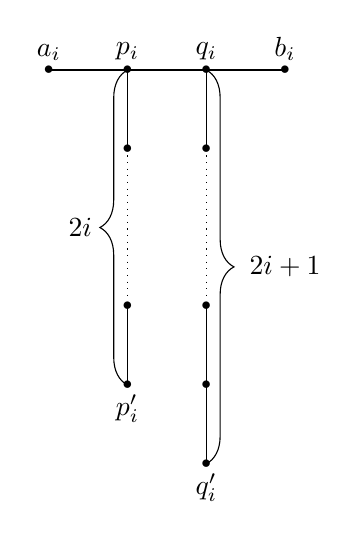
\begin{tikzpicture}
        % nodes
        \node[scale=0.7] (ai) at (0,0) {$\bullet$};
        \node[scale=0.7] (p1) at (1,0) {$\bullet$};
        \node[scale=0.7] (q1) at (2,0) {$\bullet$};
        \node[scale=0.7] (bi) at (3,0) {$\bullet$};
        \node[scale=0.7] (p2) at (1,-1) {$\bullet$};
        \node[scale=0.7] (q2) at (2,-1) {$\bullet$};
        \node[scale=0.7] (p3) at (1,-3) {$\bullet$};
        \node[scale=0.7] (q3) at (2,-3) {$\bullet$};
        \node[scale=0.7] (p4) at (1,-4) {$\bullet$};
        \node[scale=0.7] (q4) at (2,-4) {$\bullet$};
        \node[scale=0.7] (q5) at (2,-5) {$\bullet$};
        % labels
        \draw (ai) node[above]{$a_i$};
        \draw (p1) node[above]{$p_i$};
        \draw (q1) node[above]{$q_i$};
        \draw (bi) node[above]{$b_i$};
        \draw (p4) node[below]{$p_i'$};
        \draw (q5) node[below]{$q_i'$};
        \draw[decorate,decoration={brace,amplitude=10pt, mirror}, xshift = -0.3cm] (p1.center) -- (p4.center)
        node[midway, xshift = -0.6cm]{$2i$};
        \draw[decorate,decoration={brace,amplitude=10pt}, xshift = 0.3cm] (q1.center) -- (q5.center) node[midway,
        xshift=1cm]{$2i+1$};
        % edges
        \draw (ai.center) -- (p1.center) -- (q1.center) -- (bi.center);
        \draw (p1.center) -- (p2.center) (q1.center) -- (q2.center);
        \draw[dotted] (p2.center) -- (p3.center) (q2.center) -- (q3.center);
        \draw (p3.center) -- (p4.center) (q3.center) -- (q4.center) -- (q5.center);
      \end{tikzpicture}
    \end{center}
    Si $i \neq j$, on a que $T_i \not\cong T_j$, car on n'a pas le même nombre de sommets dans $T_i$ et
    $T_j$. On doit montrer que $Aut(T_i) = \{id\}$ (exercice). 

    Dans le graphe de Cayley $X_0$, on remplace chaque arête $s_i$ par $T_i$, par exemple
    \begin{center}
      \begin{tikzpicture}
        % nodes
        \node[scale=0.7] (ai) at (0,0) {$\bullet$};
        \node[scale=0.7] (p1) at (1,0) {$\bullet$};
        \node[scale=0.7] (q1) at (2,0) {$\bullet$};
        \node[scale=0.7] (bi) at (3,0) {$\bullet$};
        \node[scale=0.7] (p2) at (1,-1) {$\bullet$};
        \node[scale=0.7] (q2) at (2,-1) {$\bullet$};
        \node[scale=0.7] (p3) at (1,-3) {$\bullet$};
        \node[scale=0.7] (q3) at (2,-3) {$\bullet$};
        \node[scale=0.7] (p4) at (1,-4) {$\bullet$};
        \node[scale=0.7] (q4) at (2,-4) {$\bullet$};
        \node[scale=0.7] (q5) at (2,-5) {$\bullet$};
        % labels
        \draw (ai) node[above]{$g$};
        \draw (bi) node[above]{$gs_i$};
        % edges
        \draw[->, >=latex] (ai.center) --  (bi.center);
        \draw (p1.center) -- (p2.center) (q1.center) -- (q2.center);
        \draw[dotted] (p2.center) -- (p3.center) (q2.center) -- (q3.center);
        \draw (p3.center) -- (p4.center) (q3.center) -- (q4.center) -- (q5.center);
        % other
        \draw (-6, -2.5) node[scale=0.7]{$\bullet$} node[above]{$g$};
        \draw (-3, -2.5) node[scale=0.7]{$\bullet$} node[above]{$gs_i$};
        \draw[->, >=latex] (-6, -2.5) to node[midway, above]{$s_i$} (-3, -2.5);
        \draw[->, >=latex] (-2, -2.5) to[bend left] (0, -2.5);
      \end{tikzpicture}
    \end{center}
    et on obtient un graphe $X$. On a ainsi une expansion de $X_0$ vers $X$ ainsi qu'une contraction de $X$
    vers $X_0$ (en remplaçant $T_i$ par $s_i$). On observe que chaque automorphisme $\phi: X \to X$ induit un
    automorphisme $\phi_0: X_0 \to X_0$. 
    \begin{enumerate}
    \item Si $\gamma \in Aut(X)$ fixe $x \in V(X)$ ($\gamma(x) = x$), alors $\gamma = id_X$. En effet, si $x
      \in V(X) \setminus V(X_0)$ et $\gamma(x) = x$, alors $x \in V(T_i) \setminus \{a_i, b_i\}$. Ainsi
      $\gamma(T_i) = T_i$. Supposons que $x \in V(X_0)$ et $\gamma(T_{x,j}) = T_{x,j}$ pour chaque $x \in
      T_{x,j}$. L'idée est que si on fixe un tel $x$, on est obligé de fixer l'arbre $T_{x,j}$ (car deux
      arbres différents ne sont pas isomorphes), ainsi on fixe tous les arbres, donc toutes les arêtes et
      ainsi on fixe $xs_i$ pour chaque $i$, et par le Lemme de Zorn (car c'est un arbre infini, donc on doit
      faire ce processus à l'infini), on fixe l'arbre. C'est-à-dire que $\gamma(X) = X$, donc $\gamma = id$.

    \item $Aut(X) \cong G$. Soit $\phi: G \to Aut(X)$, $g \mapsto \phi_g$ où $\phi_g : X \to X$ est une
      extension de $\phi_g^0: X_0 \to X_0$ et $\phi_g^0(v) = gv$ si $v \in V(X_0) = G$. Commençons par montrer
      que $\phi$ est injective. On a
      \begin{align*}
        \phi(g) = \phi(g') &\iff \phi_g(v) = \phi_{g'}(v)\\
        &\iff gv = g'v\\
        &\iff g = g'
      \end{align*}
      Montrons à présent que $\phi$ est surjective. Soit $\psi \in Aut(X)$ avec $\psi(v) = v'$ pour $v,v' \in
      X_0$, alors il existe $g \in G$ tel que $\phi_g(v) = v'$ (par exemple on prend $g = v'v^{-1}$). On a
      $\psi(v) = \phi_g(v)$, et ainsi $(\psi^{-1}\phi_g)(v) = v$ et par la première observation,
      $\psi^{-1}\phi_g = id$ et donc $\psi = \phi_g$. \qedhere
    \end{enumerate}
  \end{preuve}

  \begin{rem}
    Si on change l'ensemble $S$, les graphes de Cayley pour $G$ sont différents entre eux (c'est-à-dire qu'ils
    ne sont pas isomorphes, en général). Mais ils sont \emph{quasi-isométriques} \index{Graphe!quasi-isométrique}
  \end{rem}


  À présent, on supposera toujours que $S$ engendre $G$ (sinon le graphe n'est pas connexe, et on n'a pas des
  bonnes propriétés).

  \begin{defi} \index{Longueur d'un mot $g$}
    Soit $g \in G$. La \emph{longueur} des mots de $g$ est la distance de $g$ à $\epsilon$ dans $\Gamma(G,S)$.
      \[|g|_S := \min\{n \in \N\ |\ g = s_1\cdots s_n,\ s_i \in S\}.\]

    Pour $g \in G$, la \emph{distance} de $x$ a $y$ \index{distance entre deux mots} est celle dans
    $\Gamma(G,S)$, notée $d_S(x,y) = |x^{-1}y|_S$.
  \end{defi}

  \begin{obss}
    \begin{enumerate}
    \item $d_S: G \times G \to \N$ est une distance sur $G$, invariante par l'action à gauche de $G$, $d_S(gx,
      gy) = d_S(x,y)$.

    \item Cette distance dépend du choix d'un système de générateurs $S$. Mais on va voir qu'en regardant le
      groupe \og de loin\fg, plusieurs propriétés importantes ne dépendent pas de $S$ (Gromov, $\sim 1980$).
    \end{enumerate}
  \end{obss}

  \begin{ex}
    Considérons $G = \Z$ et $S = \{\pm 1\}$. Le graphe de Cayley est simplement une droite infinie à gauche et
    à droite. Si à présent on considère $S' = \{\pm 2, \pm 3\}$, le graphe de Cayley devient 
    \begin{center}
    
            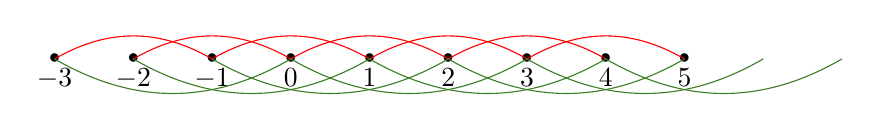
\begin{tikzpicture}
              \foreach \k in {-3,-2,...,5} { \draw (\k, 0) node[scale=0.8]{$\bullet$} node[below]{$\k$}; }
              \foreach \k in {-3, -2, ..., 3}{ \draw[color = red] (\k, 0) to[bend left] ({\k+2}, 0); }
              \foreach \k in {-3, -2, ..., 4}{ \draw[color = OliveGreen] (\k, 0) to[bend right] ({\k+3}, 0); }
            \end{tikzpicture}

          \end{center}
  \end{ex}



  \section{Quasi-isométries}
  \label{sec:quasi-isometries}

  
  Soient $(X, d)$, $(X', d')$ deux espaces métriques.

  \begin{defi}
    Une application $f: X \to X'$ est une \emph{quasi-isométrie} \index{Quasi-isométrie} s'il existe $g: X' \to
    X$ et des constante $\lambda >0$, $c \geq 0$ telles que
    \begin{enumerate}
    \item $d'(f(x), f(y)) \leq \lambda d(x,y) + c$ pour tous $x, y \in X$;
    \item $d(g(x'), g(y')) \leq \lambda d'(x', y') + c$ pour tous $x', y' \in X'$;
    \item $d(g(f(x)), x) \leq c$ pour tout $x \in X$;
    \item $d'(f'(g'(x')), x') \leq c$ pour tout $x' \in X'$.
    \end{enumerate}
    Les deux premières inégalités disent que $f, g$ sont Lipschitzienne à grande échelle. Les deux dernières
    disent que $f, g$ sont \emph{quasi-inverses} \index{Quasi-inverses} l'une de l'autre.
    On dit que $(X, d)$ et $(X', d')$ sont \emph{quasi-isométriques} \index{Espaces!quasi-isométriques} s'il
    existe une quasi-isométrie $f: X \to X'$.
  \end{defi}


  \begin{exs}
    \begin{enumerate}
    \item Soit $X = \R$ et $X' = \Z$. Considérons $f(x) = [x]$ (partie entière de $x$). Alors $f$ une
      quasi-isométrie (qi) avec $\lambda = c = 1$.

    \item Un espace borné est qi à un point (si on regarde l'espace de très très loin, il est réduit à un
      point).
    \item \textbf{Exercice:} Être qi est une relation d'équivalence parmi les espaces métriques.
    \end{enumerate}
  \end{exs}


  \begin{prop}
    Soient $S, T$ deux parties génératrices finies de $G$. Les espaces $\Gamma(G, S)$ et $\Gamma(G, T)$ sont qi.
  \end{prop}

  \begin{preuve}
    L'idée de la preuve est que chaque $s \in S$ est un mot dans $T$.
  \end{preuve}


  \begin{prop}
    Soit $G$ un groupe et $H \leq G$ un sous-groupe de $G$ d'indice fini ($|G:H| < \infty$). Alors $G$ et $H$
    sont qi.
  \end{prop}

  \begin{preuve}
    On démontrera ce résultat comme corollaire d'autres résultats plus généraux.
  \end{preuve}

  
  
  \section{Actions propres}
  \label{sec:actions-propres}

  \begin{defi}
    Soit $G$ un groupe agissant par homéomorphismes sur un espace topologique séparé $X$. L'action de $G$ sur
    $X$ est \emph{propre} \index{Action!propre} si pour tout $K, L \subset X$ parties compactes 
      \[\left| \{g \in G\ |\ gK \cap L \neq \varnothing \}\right| < \infty.\]
    Intuitivement, on ne peut pas avoir une infinité d'élément des copies de $K$ par l'action de $G$ qui
    intersecte $L$.
  \end{defi}

  \begin{prop}
    Supposons que $K = L = \{x\}$, on voit que dans une action propre, tout stabilisateur est fini.
      \[\mathrm{Stab}_G(x) = \{g \in G | gx = x\}.\]
  \end{prop}

  \begin{preuve}
    En fait on a que
    {
      \begin{align*}
        \{gx\} \cap \{x\} \neq \varnothing &\iff \{gx\} \cap \{x\} = \{x\}\\
        & \iff gx = x
      \end{align*}}
    et donc c'est assez clair.
  \end{preuve}


  \begin{exs}
    \begin{enumerate}
    \item Toute action d'un groupe fini est propre.
    \item Si $G$ agit sur $X$ avec $X$ compact, l'action est propre si et seulement si $G$ est fini. Il suffit
      de prendre $K = L = X$.
    \item L'action de $\Z^n$ sur $\R^n$ par translations est propre. 

      \textbf{Preuve:} Soient $K, L \subset \R^n$ deux parties compactes. Soit $v$ tel que $(v + K) \cap L
      \neq \varnothing$ (ici on travaille avec des vecteurs, donc la translation est représentée par le
      "+"). si et seulement s'il existe $k \in K$ et $l\in L$ tels que $v + k = l$ ss'il existe $k \in K$ et
      $l \in L$ tels que $v = l-k$ si et seulement si $v \in L \setminus K$ ($L \setminus K = C$ est
      compact). Alors $v \in C \cap \Z^n$ est fini, ce qui conclut. \qed

    \item Si $X$ est discret, l'action de $G$ sur $X$ est propre si et seulement si tous les stabilisateurs
      sont finis.

      \textbf{Preuve:} Montrons que si tous les stabilisateurs sont finis, alors l'action de $G$ sur $X$ est
      propre. Si $K, L \subset X$ sont compacts, alors ils sont finis. On peut donc écrire $K = \{x_1, \ldots,
      x_m\}$ et $L = \{y_1, \ldots, y_n\}$. On a 
      {
        \begin{align*}
          gK \cap L \neq \varnothing & \iff \exists i,j \text{ tq } gx_i = y_j.
        \end{align*}
      }
      $\{g \in G | gx_i = y_j\}$ est fini; c'est une classe latérale de $\mathrm{Stab}_G(x_i)$. \qed

    \item \textbf{Exercice:} Soit $G$ un groupe agissant par multiplication à gauche sur $(X, d)$, on pose
      $\delta(Gx, Gy) = \inf\{d(gx, hy)\ |\ g, h \in G\}$. Montrer que $\delta$ est une distance sur l'espace
      des orbites $_G \diagdown ^X$ qui définit la topologie quotient.
    \end{enumerate}
  \end{exs}




  \begin{defi} \index{Espace!géodésique}
    Un espace métrique $(X, d)$ est \emph{géodésique} si pour tous $x, y \in X$ avec $\Delta = d(x,y)$, il
    existe $\gamma:[0, \Delta] \to X$ continue avec $\gamma(0) = x$, $\gamma(\Delta) = y$, et $d(\gamma(s),
    \gamma(t)) = |s-t|$ pour tous $s, t \in [0, \Delta]$. C'est équivalent à dire que deux points quelconques
    peuvent être joints par un chemin géodésique, c'est-à-dire une isométrie d'un intervalle de $\R$ dans $X$.
  \end{defi}

  \begin{exs}
    \begin{enumerate}
    \item $\R^n$ muni de la distance euclidienne est un espace géodésique.
    \item Tous les espaces normés sont géodésiques.

      \textbf{Preuve:} Soit $X$ un espace normé et soit $\Delta = \|x - y\|$. On prend $\gamma(t) = x +
      \frac{t}{\Delta}(y-x)$, et donc $\|\gamma(s) - \gamma(t)\| = \frac{|s-t|}{\Delta}\|y-x\| = |s-t|$. \qed

    \item $\R^2$ muni de la norme $\|(x_1, x_2)\| = |x_1| + |x_2|$ n'est pas uniquement géodésique,
      c'est-à-dire qu'il existe en général plusieurs chemins géodésiques entre deux points.

    \item $\R^2 \setminus \{(0,0)\}$ muni de la métrique euclidienne n'est pas géodésique.

      
    \item Un graphe étant un espace métrique discret se plonge de manière canonique dans un espace géodésique,
      sa \emph{réalisation géométrique} \index{Réalisation géométrique} obtenue en remplaçant chaque arête par
      une copie isométrique de l'intervalle $[0,1]$.

      
    \item[5'.] Les graphes de Cayley $\Gamma(G, S)$, $\langle S \rangle = G$ sont des espaces géodésiques.
    \end{enumerate}
  \end{exs}
  
 

  \section{Théorème fondamental de la théorie géométrique des groupes}
  \label{sec:thm-fond-theorie-geom-groupes}


  \begin{theo}[Efremovich (1953), \v{S}varc (1959), Milnor (1968)] \label{thm:milnor-svarc} \index{Théorème!de Milnor-\v{S}varc}
    Soit $X$ un espace métrique géodésique, dont les boules fermées sont compactes. Soit $G$ un groupe
    agissant proprement par isométries sur $X$ avec $_G\diagdown^X$ compact. Alors $G$ est finiment engendré
    et quasi-isométrique à $X$. \href{https://392c.wordpress.com/2009/02/09/thesvarc-milnor-lemma/}{Lemme de Milnor-\v{S}varc}
  \end{theo}


  \begin{ex}
    Soit $X = \R^n$ et $G = \Z^n$. On a une action propre de $\Z^n$ sur $\R^n$ par translations. En effet
    $\R^n$ est un espace géodésique, les boules fermées sont compactes et les translations sont des
    isométries. Le quotient est compact et donc on a que $\Z^n$ est finiment engengré et quasi-isométrique à
    $\R^n$. 
  \end{ex}

  \begin{preuve}[de \ref{thm:milnor-svarc}]
    Soit $\pi: X \to _G\diagdown^X,\ x \mapsto Gx$ (orbite de $x$) la projection canonique. On met sur
    $_G\diagdown^X$ la métrique $\delta(Gx, Gy) = \inf\{d(gx,hy)\ |\ g,h \in G\} = \inf\{ d(kx, y)\ |\ k \in
    G\}$. Comme $_G\diagdown^X$ est compact, le diamètre de $_G\diagdown^X$ est fini. Posons
      \[R := \sup\{\delta(Gx, Gy)\ |\ Gx, Gy \in _G\diagdown^X \} < \infty.\]
    Soit $x_0 \in X$ un point-base, et $B = B(x_0, R)$ la boule centrée en $x_0$ centrée en $R$. Soit $S = \{s
    \in G\ |\ s \neq 1, sB \cap B \neq \varnothing\}$, qui est un ensemble fini à cause de l'action propre de
    $G$, et de plus $S$ est symétrique. Intuitivement, $S$ représente les translations de $B$ qui intersectent
    $B$. Posons encore $r := \{ \inf\{ d(B, gB)\ |\ g \notin S \cup \{1\}\}$. Ce $r$ est la plus petite
    distance entre un $B$ est une translation de $B$  qui n'intersecte pas $B$.

    \paragraph{Assertion 1:} En fait, on a $r = \min\{ d(B, gB)\ |\ g \notin S \cup \{1\}\} > 0$. En effet,
    soit $g' \in G$, $g' \notin S \cup \{1\}$; soit $r' = d(B, g'B) > 0$. Posons alors $T = \{g \in G\ |\ g
    \notin S \cup \{1\},\ d(B, gB) \leq r'\}$. $T' \neq \varnothing$ car $g' \in T$. On va voir que $T$ est
    fini. $T$ est fini car $T \subset \{g \in G\ \ gB(x_0, R+r') \cap B(x_0, R+r') \neq \varnothing\}$ qui est
    fini. En effet, il existe $x \in B$ et $g \in T$ tel que $d(x, gx) \leq r'$, donc si $x \in B$, $x \in
    B(x_0, R+r')$ et $d(x_0, gx) \leq d(x_0, x) + d(x, gx) \leq R + r'$. Ainsi $gx \in B(x_0, R+r')$. Ceci
    montre que $gx \in B(x_0, R+r') \cap gB(x_0, R + r')$. Comme $r$ est l'infimum des nombres $d(B, gB) > 0$,
    pris sur $T$ qui est fini, on a $r > 0$.

    \begin{center}
      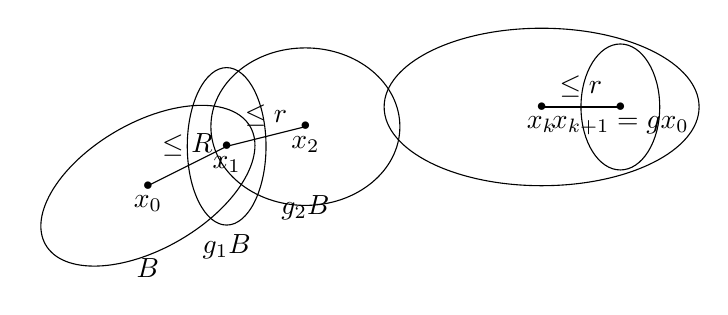
\begin{tikzpicture}
        \draw (0,0) node[scale=0.7]{$\bullet$} node[below]{$x_0$};
        \draw (1, 0.5) node[scale=0.7]{$\bullet$} node[below]{$x_1$};
        \draw (2, 0.75) node[scale=0.7]{$\bullet$} node[below]{$x_2$};
        \draw (5, 1) node[scale=0.7]{$\bullet$} node[below]{$x_k$};
        \draw (6, 1) node[scale=0.7]{$\bullet$} node[below]{$x_{k+1} = gx_0$};
        \draw (0,0) to node[midway, above]{$\leq R$} (1, 0.5) to node[midway, above]{$\leq r$} (2, 0.75);
        \draw (5,1) to node[midway, above]{$\leq r$} (6, 1);
        \draw[rotate=30] (0,0) ellipse (1.5cm and 0.8cm);
        \draw (1, 0.5) ellipse (0.5cm and 1cm);
        \draw (2, 0.75) ellipse (1.2cm and 1cm);
        \draw (5, 1) ellipse (2cm and 1cm);
        \draw (6, 1) ellipse (0.5cm and 0.8cm);
        \draw (0, -0.8) node[below]{$B$};
        \draw (1, -0.5) node[below]{$g_1B$};
        \draw (2, 0) node[below]{$g_2B$};
      \end{tikzpicture}
    \end{center}

    \paragraph{Exercice:} $r \leq 2R$.

    Soit $\lambda = \max_{s \in S}\{d(x_0, sx_0)\}$.

    \paragraph{Assertion 2:} $S$ engendre $G$ et $(\ast)$ $\frac{1}{\lambda} d(x_0, gx_0) \leq |g|_S \leq
    \frac{1}{r}d(x_0, gx_0) + 1$. Soit $g \in G$. Si $g \in S \cup \{1\}$, $(\ast)$ est clair. Si $g \notin S
    \cup \{1\}$, soit $k$ l'unique entier $\geq 0$ tel que $R + (k-1)r \leq d(x_0, gx_0) \leq R + kr$
    $(\ast\ast)$. Ce $k$ existe car $d(x_0, gx_0) > R$. Comme $X$ est géodésique, on peut trouver $x_1,
    \ldots, x_k, x_{k+1} = gx_0$ dans $X$ avec $d(x_0, x_1) \leq R$ et $d(x_i, x_{i+1}) < r$ pour $i = 1,
    \ldots k$. Ceci marche car on a $d(x_0, gx_0) \leq R + kr$, qui est ce qu'on veut. Comme $X = \bigcup_{g
      \in G} gB$, on peut choisir $g_0 = 1, g_1, \ldots, g_k = g$ tels que $x_i \in g_{i-1}B$ pour $i = 1,
    \ldots, k$. On pose $s_i = g_{i-1}^{-1}g_i$, ce qui veut dire que $s_ig_i^{-1} = g_{i-1}^{-1}$ et donc $g = s_1s_2\cdots s_k$. On a $d(B, s_iB) \leq
    d(g_{i-1}^{-1}x_i, s_ig_i^{-1}x_{i+1}) = d(x_i, x_{i+1}) < r$. Par définition de $r$, $s_i \in S \cup
    \{1\}$ et donc $S$ engendre $G$! (On a $g_{i-1}^{-1} x \in B$ car $x \in g_{i-1}B$.) Pour la fin de la
    preuve, voir feuille annexe.

    \textbf{Observation:} $d(x_0, g^{-1}hx_0) = d(gx_0, hx_0)$ (car la distance est invariante par actions à
    gauche). Ceci est la distance entre deux points dans l'orbite.

    Ainsi $(\ast)$ nous donne que
      \[\frac{1}{\lambda} d(gx_0, gx_0) \leq d_S(g, h) \leq \frac{1}{r} d(gx_0, hx_0) + 1,\]
    ce qui se traduit par le fait que $G$ est qi à l'orbite $Gx_0$, avec la métrique induite par $d$.

    \paragraph{Assertion 3:} L'inclusion $f: Gx_0 \hookrightarrow X$ est une quasi-isométrie. On définit $f':
    X \to Gx_0$ en envoyant un point $x \in X$ sur un point $x'$ de $Gx_0$ à distance $\leq R$ de $x$, avec
    $f'(x)=x$ si $x \in Gx_0$. Alors
      \[d(x,y) - 2R \leq d(f'(x), f'(y)) \leq d(x,y) + 2R.\]
      \begin{center}
      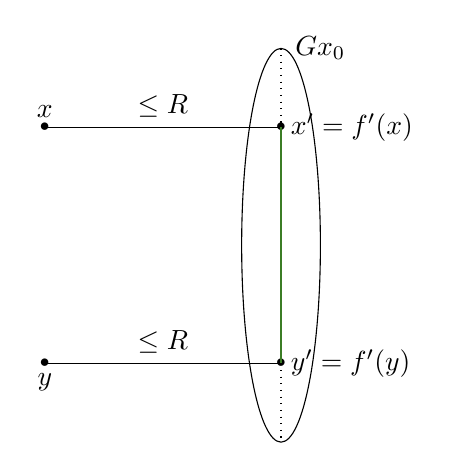
\begin{tikzpicture}
        \draw (0,0) node[scale=0.7]{$\bullet$} node[above]{$x$};
        \draw (3,0) node[scale=0.7]{$\bullet$} node[right]{$x' = f'(x)$};
        \draw (0,-3) node[scale=0.7]{$\bullet$} node[below]{$y$};
        \draw (3,-3) node[scale=0.7]{$\bullet$} node[right]{$y' = f'(y)$};
        \draw (0,0) to node[midway, above]{$\leq R$} (3, 0);
        \draw (0,-3) to node[midway, above]{$\leq R$} (3, -3);
        \draw[color=OliveGreen] (3, 0) -- (3, -3);
        \draw[dotted] (3,1) -- (3,0) (3, -3) -- (3, -4);
        \draw (3, -1.5) ellipse (0.5cm and 2.5cm);
        \draw (3.5, 1) node {$Gx_0$};
      \end{tikzpicture}
    \end{center}
    On a que $f' \circ f = Id_{Gx_0}$, car si $x \in Gx_0$, alors $f'(f(x)) = x$. De plus $d(x, f(f'(x)) \leq
    R$, car pour tout $x \in X$, $f'(x) = x'$, $f(f'(x)) = f(x') = x'$. Ceci termine la preuve, car ainsi $f$
    et $f'$ sont des qi.
  \end{preuve}


  \begin{cor}
    Soit $G$ un groupe finiment engendré et soit $H$ un sous-groupe d'indice fini. Alors $H$ est finiment
    engendré, et qi à $G$.
  \end{cor}

  \begin{preuve}
    Exercice.
  \end{preuve}

  

  

  




%%% Local Variables:
%%% mode: latex
%%% TeX-master: "../GAC_cours.tex" 
%%% End: